\documentclass{ubo_tex_uebungszettel/uebungszettel}
\vorlesung{Python Vertiefungskurs}
\semester{SoSe 2023}
\author{Chris Geron}
\assi{}
\tutor{
Adrian~Oeyen,
Mathilde~Schreck
}


\renewcommand{\itswg}{false}

\usetikzlibrary{fit, positioning, shapes.geometric, shapes.misc}

\newcommand{\tb}[1]{\textbf{#1}}

\definecolor{colorblue}{HTML}{07529A}   % Uni Blau 100%
\definecolor{colorgray}{HTML}{909085}   % Unigrau
\definecolor{coloryellow}{HTML}{eab90c} % Unigelb

%
% Ablaufdiagram
%
\tikzstyle{startstop} = [draw, rounded rectangle, text centered, draw=black,thick]
\tikzstyle{io} = [draw, trapezium, trapezium left angle=70, trapezium right angle=110, text centered]
\tikzstyle{process} = [rectangle, text centered, draw=black,thick]
\tikzstyle{decision} = [diamond, aspect=1.5, text centered, draw=black,thick]


%
% Bäume zeichnen
%
\tikzstyle{baum} = [
  every node/.style={fill=coloryellow!25, minimum size=1.5ex, thick, draw=black, text=black},
  every edge/.style={thick, draw=black}
]

\tikzset{
  tri/.style={
    draw,
    isosceles triangle,
    isosceles triangle apex angle=22,
    shape border rotate=90,
    inner sep=0.1pt,
    minimum width=0.5cm,
  }
}

% UML Diagramme
\providecommand{\umltextcolor}{}
\providecommand{\umlfillcolor}{}
\providecommand{\umldrawcolor}{}
\renewcommand{\umltextcolor}{colorblue}
\renewcommand{\umlfillcolor}{coloryellow!20}
\renewcommand{\umldrawcolor}{coloryellow}

\tikzstyle{classdiag} = [
  every node/.style = {font=\footnotesize}
]


\newcommand{\lazytt}[1]{
\smallskip
\noindent\fbox{
  \centering
  \parbox{\dimexpr\linewidth-2\fboxsep-2\fboxrule\relax}{
    \footnotesize\texttt{#1}
  }
}\smallskip
}




\title{Zettel 02}
\ausgabe{12. September 2023}
\abgabe{}
\hinweis{}


\theoremstyle{definition}
\newtheorem*{story}{Story}

\newcommand{\pp}[1]{\lpl{#1}}
\newcommand{\furl}[1]{\footnote{\url{#1}}}

\begin{document}

\maketitle

\noindent \tb{Hinweis}: \quad
Dieser Zettel enthält mehr Aufgaben, als vermutlich innerhalb des Tutoriums machbar sind.\\
Schauen Sie sich die Aufgaben an und bearbeiten Sie zuerst die Aufgaben, welche Sie ansprechen.\\
Fühlen Sie sich frei, gegebene Aufgaben um beliebige Funktionaliät zu erweitern oder zu modifizieren.

\medskip

\noindent In einigen Aufgaben finden Sie Referenzen zu bereits vorbereiteten Programmen. Diese können Sie aus diesem Sciebo-Share\furl{https://uni-bonn.sciebo.de/s/eADQTyhzRLkFSi6} im Ordner des entsprechenden Tages finden und runterladen.

\medskip


\noindent \tb{Entwicklungsumgebung aufsetzen} \quad

    \begin{enumerate}
        \item Falls dies nicht bereits an einem vorherigen Tag geschehen ist, setzen Sie sich ein Virtual Environment und eine Entwicklungsumgebung auf.\\
        Mehr dazu finden Sie auf Zettel 1.

        \item Erweritern Sie ihr \pp{venv} um die Packages \pp{fastapi} und \pp{requests}.
    \end{enumerate}

\medskip
\medskip

\medskip
\noindent \tb{Wiki-Race} \quad
  
    \noindent
    Das Wikipedia-Game beinhaltet das Ziel, von einem Startartikel aus nur durch das Klicken auf Verlinkungen in den Artikeln den schnellsten Weg zu einem vorher festgelegten Zielartikel zu finden. \\
    \noindent Sie sollen das Spiel nun für die Konsole implementieren.
    Beginnend bei dem Artikel zu \texttt{Königspython} sollen auf der Konsole alle möglichen Links angezeigt bekommen.\\

    \medskip 
    \noindent Dafür können Sie diese vorgefertigte URL der Wikipedia API\footnote{\url{https://de.wikipedia.org/w/api.php?action=query&prop=links&pllimit=max&format=json&titles=SUCHBEGRIFF}} verwenden.

    \noindent Per \texttt{input()} kann der gewünschte nächste Artikel aus der gezeigten Auswahl gewählt werden.\\
    Das Programm soll dann die die neuen Links der entsprechenden Seite laden und anzeigen.\\
    \medskip
    Das Spiel ist gewonnen, sobald der Artikel \texttt{Python (Programmiersprache)} erreicht ist.


\pagebreak

\medskip
\noindent \tb{Ein Programm Packaging} \quad


    \noindent Ziel der Aufgabe ist es, ein Programm Ihrer Wahl in ein aus der Kommandozeile ausführbares Programmm zu paketieren. Die Aufgabe ist sehr kleinschrittig aufgegliedert und wirkt daher nach mehr als sie eigentlich ist.
    \begin{enumerate}
        % TODO Gitlab
        \item Laden Sie sich das \pp{PyPa sample project}\furl{https://github.com/pypa/sampleproject/archive/refs/heads/main.zip} runter.
        \item Entpacken Sie es an einen Ort, wo es Ihnen gut passt.
        \item Geben Sie dem Package einen sinnvollen Namen.
        \item Fügen Sie ein Programm - z.B. Ihre Wiki Race Implementation - in \pp{simple.py} ein (Benennen Sie auch diese Datei gerne um!).
        \item[] Wichtig ist hierbei, dass alle Funktionaitäten in Funktionen (oder Klassen) verpackt sind und das Programm durch den Aufruf einer Funktion startbar ist.
        \item Importieren Sie ihre Start-Funktion in die \pp{__init__.py} und rufen Sie diese in der \pp{main()} auf.
        \item Passen Sie die \pp{pyproject.toml} so an, dass die Metadaten den Angaben zu Ihrem Projekt entsprechen. (Löschen Sie, nicht benötigte, optionale, Inhalte einfach raus.)
        \item[] Passen Sie hierbei insbesondere den Namen Ihres Kommandozeilenprogramms\\ \pp{[project.scripts]} an.
        \item Öffnen Sie ein Terminal, stellen Sie sicher, dass Sie im Wurzelverzeichnis Ihres Projekts sind und Ihr \pp{venv} aktiviert haben\furl{https://docs.python.org/3/library/venv.html\#how-venvs-work}\footnotetext{Das \texttt{venv} muss nicht im selben Verzeichnis liegen. Sie können das Verzeichnis auch nach aktivieren des \texttt{venv} beliebig wechseln.}.
        \item Installiere Sie Ihr Package mit \pp{python3 -m pip install -e .}
        \item Rufen Sie das von Ihnen erstellte Kommandozeilenprogramm auf.
    \end{enumerate}

    \medskip
    \noindent \tb{Typehinting} \quad
    
        \noindent Ziel der Aufgabe ist es, Sie mit den weiterführenden Konzepten des Typehintings vertraut zu machen.
        \begin{enumerate}
            \item Ergänzen Sie den Code in \pp{typehinting.py} um sinnvolle Typehints.
            \item[] Hinweis: Denken Sie an \pp{Type aliases}.
            \item Erstellen Sie Funktionen und Objekte, welche zu den weiter unten in der Datei gegebenen Typehints passen.
        \end{enumerate}

    \pagebreak
    
    \medskip
    \noindent \tb{Pydantic / Dataclasses} \quad

    \noindent In dieser Aufgabe können Sie frei wählen, ob Sie sich lieber mit \pp{Pydantic} oder \pp{dataclasses} weiter vertraut machen wollen.

    \noindent Ziel ist es, Bands und deren Mitglieder als Dataclasses zu modellieren.
    
        \noindent
        \begin{enumerate}
            \item Modellieren Sie das gegebene UML Diagram. Sie dürfen das Modell dabei um beliebige Funktionalitäten und Hilfsfunktionen ergänzen.
            \end{enumerate}
            
            Tipps zum Vorgehen:
            \begin{itemize}
                \item Achten Sie generell darauf, frühzeitig eine gute String-Repräsentation für Ihre Modelle zu haben.
                \item Modellieren Sie zunächst \pp{BandMember}.
                \item Erstellen Sie danach das grobe Design des \pp{Band}-Modells.
                \item Ergänzen Sie zuletzt die \pp{json}-Serialisierbarkeit.
            \end{itemize}
            
    \begin{figure}[h!]
        \centering
        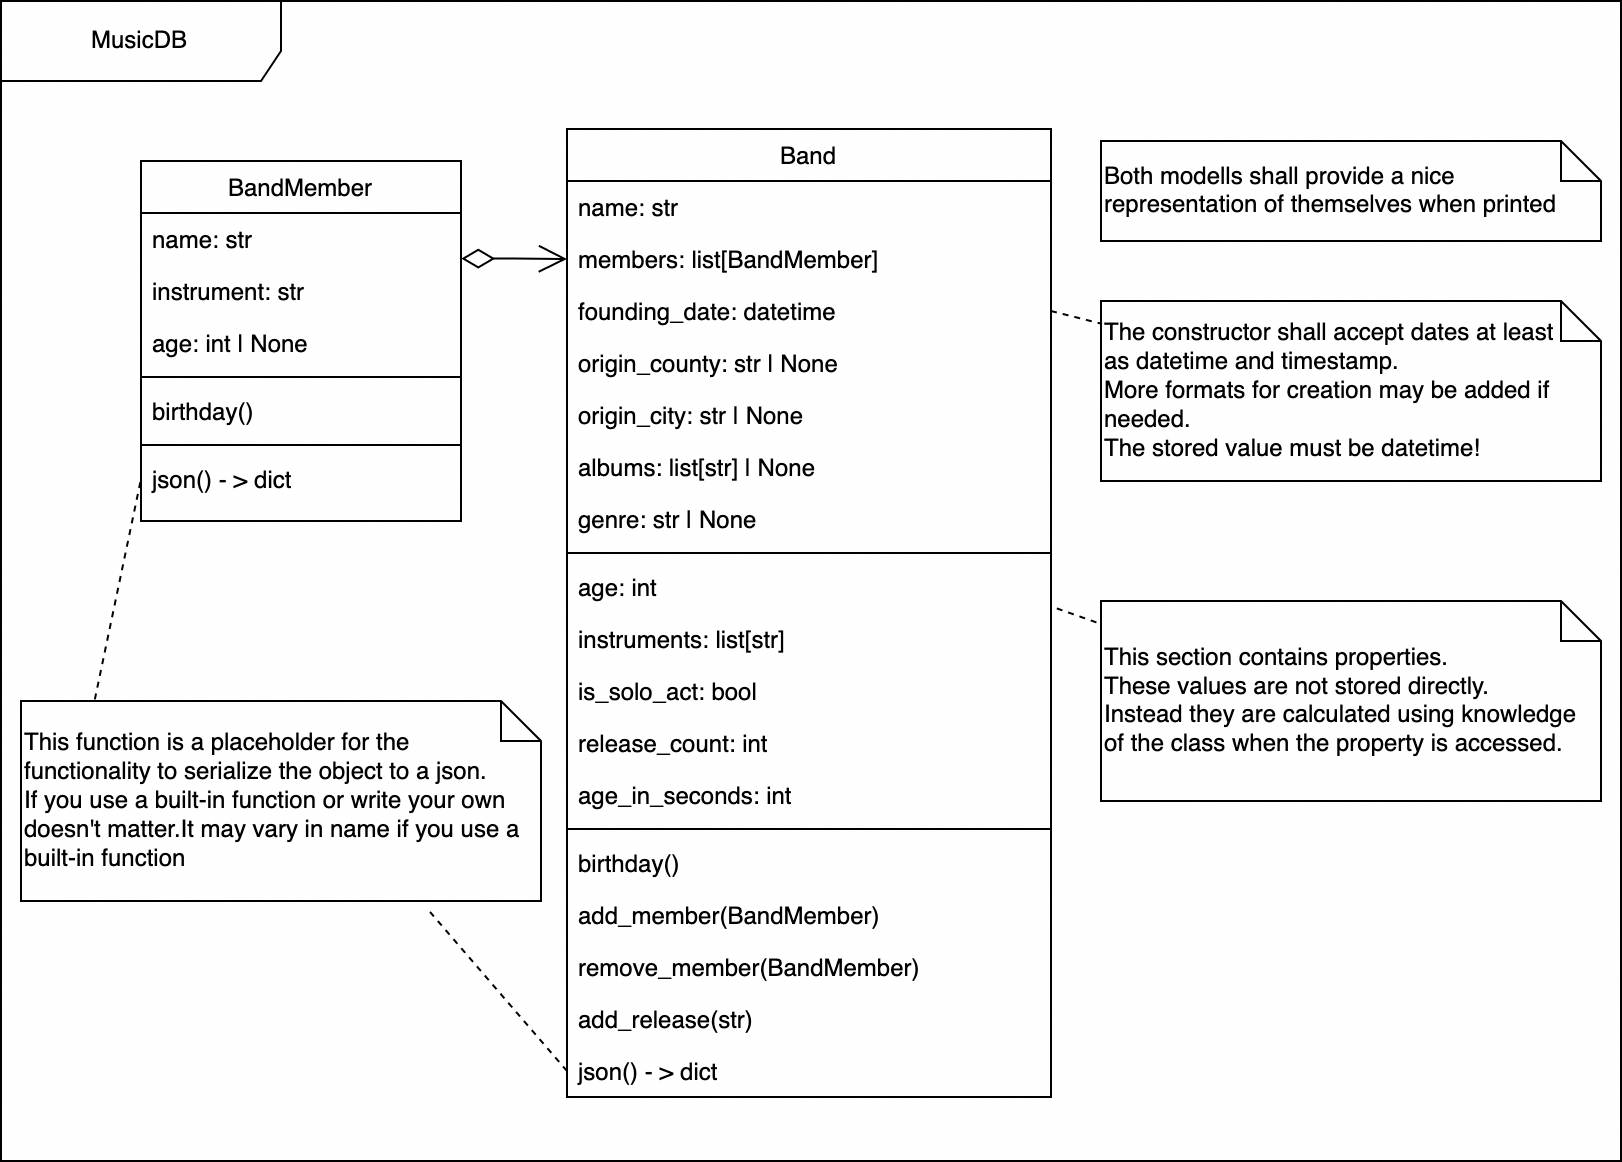
\includegraphics[width=.9\textwidth]{images/band-uml.png}
        \caption{Das zu modellierende UML-Diagram}
    \end{figure}

    \pagebreak

    \medskip
    \noindent \tb{FastAPI} \quad
    
        \noindent Ziel der Aufgabe ist es, Ihnen Ideen für eine mögliche API zu geben. Es werden im Folgenden zwei in etwa gleich komplexe Systeme vorgeschlagen.\\
        Auch hier haben Sie die freie Wahl, ob Sie für Ihre Datenmodelle \pp{Pydantic} oder \pp{dataclass} nutzen wollen.

        \noindent
        \tb{Notify}:
        \begin{itemize}
            \item Eine Route, an die Nachrichten (z.B. Text) geschickt werden kann.
            \item Der Server speichert diese Nachrichten intern ab.
            \item Eine weitere Route ermöglicht das Abholen aller hinterlegten Nachrichten.
            \item[] Mögliches Herangehen:
            \item[] \begin{itemize}
                \item Überlegen Sie sich, welchen Kontext die Nachricht noch enthalten soll.
                \item[] Soll vielleicht ein Absender, oder der Timestamp des Empfangs mit gespeichert werden? Wie wäre es mit einem eindeutigen Identifier - Stichwort \pp{uuid}?
                \item Modellieren Sie eine Datenklasse, die Ihren Vorstellungen entspricht.
                \item Definieren Sie eine Route, welche eine Nachricht engegenenehmen kann und die entsprechenden Parameter bietet.
                \item Speichern Sie die Nachrichten intern.
                \item Fügen Sie eine weitere Route hinzu, welche das Abfragen der Nachrichten ermöglicht.
                \item[] Soll es hierbei vielleicht die Option geben, nur die ersten n-Nachrichten anzufragen?
            \end{itemize}
            \item Mögliche Ergänzungen:
            \item[] \begin{itemize}
                \item Eine Route, um nur anzufragen, ob Daten vorliegen
                \item Mehrere unterschiedlich benannte Kanäle
                \item Eine Übersicht, welche Kanäle existieren (und ob Daten verfügbar sind).
            \end{itemize}
        \end{itemize}

        \medskip
        \tb{URL-Shortener}:
        \begin{itemize}
            \item Eine Route, welche das Registrieren einer URL inklusive gewünschtem Short-Link erlaubt.
            \item Eine Route, welche bei Aufruf des gekürzten Links den Originallink zurückgibt.
            \item[] Mögliches Herangehen:
            \item[] \begin{itemize}
                \item Überlegen Sie sich, welchen Kontext eine gekürzte URL noch enthalten soll.
                \item[] Soll vielleicht die erstellende Person, oder der Timestamp der Erstellung mit gespeichert werden? 
                \item Modellieren Sie eine Datenklasse, die Ihren Vorstellungen entspricht.
                \item Definieren Sie eine Route, welche eine Nachricht engegenenehmen kann und die entsprechenden Parameter bietet.
                \item Speichern Sie die Nachrichten intern.
                \item[] Wie stellen Sie sicher, dass jeder Short-Link zur einmal verfügar ist?
                \item Fügen Sie eine weitere Route hinzu, welche das Aufrufen der gekürzten Links ermöglicht.
            \end{itemize}
            \item Mögliche Ergänzungen:
            \item[] \begin{itemize}
                \item Eine Übersicht über alle gekürzten Links.
                \item[] Sollen Links explizit als unsichtbar registriert werden können?
                \item Eine Route, um Links wieder zu entfernen.
                \item[] Wie können wir sicherstellen, dass nur der Ersteller den Link löschen kann? Welche Art von eindeutigem Identifier könnte er bekommen? 
                \item Soll der Name des gekürzten Links optional sein?
                \item[] Wie könnte ein zufälliger Link generiert werden?
                \item Tricky: Wollen Sie vielleicht das Hinterlegen von Bildern erlauben?
            \end{itemize}
        \end{itemize}




\end{document}
